\begin{XeClass}{RawLocalFs}
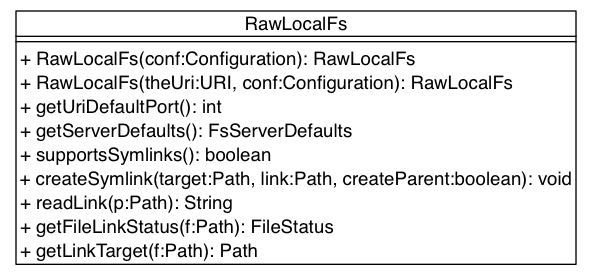
\includegraphics[width=10cm]{cdig/RawLocalFs.png}
    
    \begin{XeMethod}{\XeProtected}{int}{getUriDefaultPort}
         
 返回URI默认端口

    \end{XeMethod}

    \begin{XeMethod}{\XeProtected}{FsServerDefaults}{getServerDefaults}
         
 返回默认服务器

    \end{XeMethod}

    \begin{XeMethod}{\XeProtected}{void}{createSymlink}
         
 建立符号连接
 符号链接一般用于将一个文件或这个目录结构移动到系统中的另一个位置

    \end{XeMethod}

    \begin{XeMethod}{\XePrivate}{String}{readLink}
         
 读取建立的符号连接

    \end{XeMethod}

    \begin{XeMethod}{\XeProtected}{FileStatus}{getFileLinkStatus}
         
 获取文件连接状态

    \end{XeMethod}

    \begin{XeMethod}{\XeProtected}{Path}{getLinkTarget}
         
 获取连接目标

    \end{XeMethod}

\end{XeClass}
